\documentclass[11pt,a4paper]{article}

\usepackage[margin=1in]{geometry}
\usepackage[T1]{fontenc}
\usepackage[utf8]{inputenc}
\usepackage{lmodern}
\usepackage{microtype}
\usepackage{amsmath,amssymb,amsfonts,amsthm}
\usepackage{booktabs}
\usepackage{array}
\usepackage{enumitem}
\usepackage{graphicx}
\usepackage{hyperref}
\usepackage{xcolor}

\hypersetup{
  colorlinks=true,
  linkcolor=blue!45!black,
  citecolor=blue!45!black,
  urlcolor=blue!45!black,
  pdftitle={Valid State Transition Framework},
  pdfauthor={Martin Petrasek}
}

\setlist[itemize]{leftmargin=1.4em}
\setlist[enumerate]{leftmargin=1.6em}
\renewcommand{\arraystretch}{1.15}

\newtheorem{definition}{Definition}
\newtheorem{principle}{Principle}
\newtheorem{observation}{Observation}
\newtheorem{criterion}{Criterion}
\newtheorem{hypothesis}{Hypothesis}
\newtheorem{conjecture}{Conjecture}
\newtheorem{limitation}{Limitation}
\newtheorem{assumption}{Assumption}

\newcommand{\VST}{\mathrm{VST}}
\newcommand{\VSTR}{\mathrm{VSTR}}
\newcommand{\VSTE}{\mathrm{VSTE}}
\newcommand{\VSTJ}{\mathrm{VSTJ}}
\newcommand{\VSTF}{\mathrm{VSTF}}
\newcommand{\VIRR}{\mathrm{VIRR}}
\newcommand{\OSD}{\mathrm{OSD}}
\newcommand{\PSI}{\mathrm{PSI}}
\newcommand{\IET}{\mathrm{IET}}
\newcommand{\E}{\mathbb{E}}
\newcommand{\R}{\mathbb{R}}
\newcommand{\1}{\mathbf{1}}
\newcommand{\dd}{\mathrm{d}}
\newcommand{\Texit}{T_{\mathrm{exit}}}
\newcommand{\Treturn}{T_{\mathrm{return}}}

\title{\textbf{Valid State Transition Framework}\\
\large An Operational Standard for Stabilized Outcomes in Physical, Biological, and Computational Systems}

\author{Martin Petrasek\\
Institute for Resonant Synthesis and Field Physics (IRSFP)\\
Prague, Czech Republic\\
\href{mailto:martin.petrasek@irsfp.org}{martin.petrasek@irsfp.org}\\
ORCID: 0009-0007-4512-9528}

\date{\today}

\begin{document}
\maketitle

\begin{abstract}
Many systems are evaluated by activity-like quantities: operations per watt, signal amplitude, entropy production, risk scores, biomarker shifts, perturbation response, or transient behavioral output. These measures are often indispensable, but they do not by themselves establish that a system has produced a durable, distinguishable, and operationally meaningful outcome. A processor may dissipate energy without producing an accepted stable result; a physiological system may show changing signals without clinically actionable state transition; a tumor model may lose viability without a retained shift away from a pathological tumor-state; and a neuromodulated motor system may display evoked activity without restored voluntary control.

This manuscript introduces the \emph{Valid State Transition Framework} (VSTF), a conservative event-level measurement grammar in which the elementary unit of analysis is not raw activity but a \emph{valid stabilized state transition}. A state-valid transition is defined as a segmented movement between operationally specified state regions that satisfies localization under an observation model, distinguishability under a declared decision rule, first-exit or dwell-time stability over a declared window, and a domain-specific validity predicate. Cost-accounting completeness is reported as a separate quality flag that determines whether cost-normalized claims are allowed. The framework defines rate- and cost-normalized observables for accepted transitions, separates fully measured claims from task-level and proxy estimates, and gives falsification criteria that prevent overclaiming from transient responses or post-hoc thresholds.

VSTF does not claim to replace transition path theory, first-passage analysis, stochastic thermodynamics, clinical prediction methodology, or domain-specific mechanistic models. Its contribution is narrower and operational: it changes which dynamically detected transitions are allowed to enter the numerator of a performance, validation, or intervention metric. The central question becomes: how many pre-specified, distinguishable, retained, domain-valid transitions does a system produce per unit time, energy, perturbation, or risk exposure, including failed attempts in the appropriate denominator? This formulation yields testable protocols in hardware benchmarking, ICU time-series evaluation, cancer repair-state reset experiments, and motor-control rehabilitation studies.
\end{abstract}

\noindent\textbf{Keywords:} stabilized transitions; irreversible decisions; state validity; event-level metrics; information thermodynamics; metastability; physiological stability; cancer systems biology; neurorehabilitation; reproducibility.

\section{Motivation}

Scientific and engineering measurements often quantify \emph{activity}: power consumption, operations, events, spikes, biomarker expression, entropy production, signal amplitude, risk-score elevation, or perturbation response. Activity is necessary to understand a system, but it is not always the right unit for evaluating an outcome.

Four examples illustrate the problem.

\begin{enumerate}
  \item In hardware, high operation throughput does not guarantee that each operation corresponds to an accepted, retained, physically stable output. Energy may be spent on internal activity, failed attempts, rejected states, conversion overhead, readout, or correction.
  \item In clinical physiology, changing vital-sign dynamics may reflect destabilization, but a high dynamic score is not automatically a validated patient-level prediction, alarm, or clinical decision rule.
  \item In oncology, a perturbation may kill cells or alter expression acutely without durably moving surviving tissue away from a pathological repair-state basin after withdrawal and rechallenge.
  \item In neurorehabilitation, electrical stimulation can evoke activity without proving voluntary control, retention, or a new motor regime.
\end{enumerate}

These cases share a hidden structure: the scientifically relevant event is not raw activity, but a transition that becomes stable, distinguishable, and valid under a declared operational rule. VSTF formalizes this common structure in the spirit of systems and complexity approaches that emphasize relations, state change, and context rather than isolated scalar activity \cite{sturmberg2014}.

\section{Scope and Non-Claims}

VSTF is deliberately narrow.

\begin{itemize}
  \item It is not a theory of everything.
  \item It does not introduce a new thermodynamic law.
  \item It does not claim that one scalar metric can replace domain-specific models.
  \item It does not assert that all biological, computational, or cosmological systems share one mechanism.
  \item It does not turn retrospective associations into causal validation.
  \item It does not claim novelty for transition rates, first-passage events, metastable basins, or reactive trajectories as such.
\end{itemize}

The framework provides a measurement grammar for a specific question:

\begin{quote}
\emph{When should a change in a physical, biological, or computational system be counted as a valid state transition rather than as transient activity?}
\end{quote}

The intended contribution is therefore:
\[
  \VSTF =
  \mathrm{dynamic\ transition}
  + \mathrm{operational\ acceptance}
  + \mathrm{retention}
  + \mathrm{cost\ boundary}
  + \mathrm{pre\mbox{-}specification}.
\]

The word ``framework'' is used intentionally. A stronger theory-level claim would require additional axioms, identifiability results, or nontrivial theorems beyond the operational standard developed here.

\section{Contributions and Defensible Novelty}

The defensible novelty of VSTF is not the existence of state transitions, transition rates, first-passage times, or metastable basins. Those objects are already central in dynamical systems theory, Transition Path Theory, Markov-state modeling, reliability engineering, and clinical prediction methodology. The contribution is the \emph{acceptance layer} placed between a dynamically detected transition and a scientific claim about outcome production.

\begin{table}[h]
\centering
\caption{Nearest antecedents and the incremental VSTF layer.}
\begin{tabular}{p{0.24\linewidth}p{0.33\linewidth}p{0.33\linewidth}}
\toprule
Antecedent & What it already provides & What VSTF adds \\
\midrule
Transition Path Theory & Reactive trajectories, committors, fluxes, and transition rates between state sets. & Domain-valid outcome acceptance, retention as a reporting gate, rejected-event accounting, and claim-level restrictions. \\
First-passage and exit-time analysis & Hitting, exit, and dwell events under specified regions. & A protocol for deciding which detected events are scientifically countable as outcomes. \\
Reliability/yield metrics & Pass/fail counts and accepted outputs. & Cross-domain coupling of yield with latent-state localization, distinguishability, retention, and cost boundaries. \\
Clinical prediction standards & Calibration, discrimination, utility, external validation, and risk-of-bias assessment. & A state-transition vocabulary that prevents instability features from being called clinical events without validation. \\
Conformity assessment & Acceptance/rejection rules under measurement uncertainty, acceptance intervals, and producer/consumer risk. & Extension from static object conformity to temporally segmented dynamic transitions with retention, state semantics, rejected-event accounting, and cost-normalized reporting. \\
Stochastic thermodynamics & Trajectory-level work, heat, entropy production, and fluctuation relations. & Separation of thermodynamic dissipation from accepted stabilized outcome counts. \\
\bottomrule
\end{tabular}
\end{table}

The manuscript is therefore intended as a methodological framework with three precise claims:

\begin{enumerate}
  \item Many domains confuse activity with outcome; VSTF formalizes a conservative adjudication layer that prevents this confusion.
  \item The accepted-transition numerator and the full-boundary denominator can change rankings, interpretations, and claims relative to raw activity or raw transition counts.
  \item The framework is falsifiable because each domain claim must survive baseline comparison, locked thresholds, event segmentation, retention testing, and external or separate validation.
\end{enumerate}

More precisely, VSTF extends the logic of conformity assessment and measurement decision rules from static objects to dynamic state transitions. A static object may be accepted or rejected under measurement uncertainty; a VSTF event is accepted only after temporal segmentation, state localization, distinguishability, event-level retention, domain admissibility, and denominator accounting have all been declared.

\section{Notation}

\begin{table}[h]
\centering
\caption{Core notation used throughout the framework.}
\begin{tabular}{p{0.22\linewidth}p{0.68\linewidth}}
\toprule
Symbol & Meaning \\
\midrule
$X_t$ & Latent system state at time $t$. \\
$Y_t$ & Observed data generated from $X_t$ through measurement model $P_M(Y_t\mid X_t)$. \\
$K_\theta$ & Latent transition kernel or dynamical model used when model-based filtering is claimed. \\
$\pi_t(C_j)$ & Filtering probability $\Pr_\theta(X_t\in C_j\mid Y_{0:t})$. \\
$\mathcal{X}$ & State space. \\
$C_i$ & Operational state region or basin. \\
$e_k$ & Candidate event segment. \\
$t_{\mathrm{start}}$ & Event start time under the locked segmentation rule. \\
$t_{\mathrm{commit}}$ & First time at which the target state commitment rule is satisfied. \\
$t_{\mathrm{end}}$ & Event end time after dwell, exit, return, or refractory conditions are resolved. \\
$\epsilon$ & Localization error tolerance. \\
$\alpha$ & Distinguishability error tolerance. \\
$\delta$ & Persistence or return-failure tolerance. \\
$\tau_\ast$ & Minimum declared persistence or retention window. \\
$V_{\mathrm{dom}}$ & Pre-specified domain-validity predicate. \\
$A_k$ & Hard accepted-transition indicator for candidate event $k$. \\
$p_k$ & Posterior or estimated probability that candidate event $k$ is valid. \\
$R_k(\tau_\ast)$ & Event-level retention indicator for candidate event $k$. \\
$\rho_j(\tau_\ast)$ & Population retention reliability for target region $C_j$. \\
$Q_k^{\mathrm{acct}}$ & Accounting-quality flag for event $k$. \\
$Q_{\mathcal{B}}^{\mathrm{acct}}[a,b]$ & Window-level accounting-completeness flag for the full denominator in $[a,b]$. \\
$E_{\mathrm{sup}}^{\mathcal{B}}[a,b]$ & Full-boundary supplied energy or cost ledger over the declared window. \\
$N_{\VST}$ & Count of accepted valid stabilized transitions. \\
$\widehat{\VSTR}$ & Finite-window accepted-transition rate. \\
$\widehat{\VSTE}$ & Finite-window energy-normalized accepted-transition yield. \\
$\VSTJ$ & Perturbation-normalized accepted-transition yield. \\
$\mathcal{B}$ & System boundary for energy, dose, time, readout, rejection, and stabilization costs. \\
\bottomrule
\end{tabular}
\end{table}

\section{State Space and Operational Partitions}

Let a system be represented by a latent state variable
\[
  X_t \in \mathcal{X},
\]
where $\mathcal{X}$ may be a microscopic phase space, a coarse-grained physical state space, a vector of clinical time-series features, a molecular module space, or an experimentally defined output space.

Measurements are represented separately:
\[
  Y_t \sim P_M(\,\cdot \mid X_t),
\]
where $P_M$ is the observation model induced by the measurement map $M$, sensor noise, preprocessing, classifier, and readout procedure. This distinction prevents the probability of a latent state from being conflated with statistical confidence about that state.

When the manuscript uses a latent posterior such as $\Pr(X_t\in C_j\mid Y_{0:t})$, the observation model is not sufficient by itself. A model-based posterior also requires a prior and latent dynamics, for example
\[
  X_0\sim p_0,\qquad
  X_{t+\Delta t}\sim K_\theta(\,\cdot\mid X_t),\qquad
  Y_t\sim P_M(\,\cdot\mid X_t).
\]
Only under such a model is the filtering probability
\[
  \pi_t(C_j)=\Pr_\theta(X_t\in C_j\mid Y_{0:t})
\]
well-defined. If a study instead uses a calibrated classifier score $\Pr(C_j\mid Y_t)$, it should be reported as classifier-based localization rather than as a latent-state posterior.

\begin{definition}[Operational state region]
An operational state region is a measurable subset
\[
  C_i \subset \mathcal{X}
\]
with a declared interpretation, measurement procedure, tolerance, and resolution rule. Regions may be fixed from prior knowledge or estimated from a training/reference cohort, but they must be frozen before confirmatory evaluation.
\end{definition}

Examples include a latched digital output, a metastable attractor basin, a classified benchmark output, a high-\OSD{} tumor state, a low-\OSD{} reference state, or a motor-output state coupled to voluntary intent.

\begin{definition}[Candidate event segmentation]
A candidate event is a protocol-defined segment
\[
  e_k=(t_{\mathrm{start}},t_{\mathrm{commit}},t_{\mathrm{end}})
\]
constructed before outcome inspection. The segmentation rule must specify origin region, departure condition, target commitment condition, dwell window, hysteresis or refractory interval, and the rule by which a new event may begin.
\end{definition}

For a transition from $C_i$ to $C_j$, a typical segmentation rule is:
\[
  \mathrm{last\ exit\ from\ } C_i
  \rightarrow
  \mathrm{first\ commitment\ to\ } C_j
  \rightarrow
  \mathrm{minimum\ dwell\ or\ first\mbox{-}exit\ test}.
\]
This prevents boundary chatter or high sampling frequency from inflating event counts.

\begin{definition}[Candidate transition]
A candidate transition over an event segment $e_k$ is an observed or inferred movement
\[
  C_i \longrightarrow C_j,\qquad i \neq j,
\]
under a declared protocol $\pi$, measurement map $M$, and system boundary $\mathcal{B}$.
\end{definition}

The system boundary $\mathcal{B}$ specifies which energy, time, control, readout, rejection, and stabilization costs are charged to the transition.

\section{Assumptions Required for Confirmatory Use}

Exploratory uses of VSTF may be broader, but confirmatory claims require the following assumptions to be declared and assessed.

\begin{assumption}[Locked partition]
The state regions $C_i$, measurement map $M$, segmentation rule, tolerances $(\epsilon,\alpha,\delta,\tau_\ast)$, and domain predicate $V_{\mathrm{dom}}$ are fixed before the confirmatory outcome is inspected. If any element is tuned on the same outcome used for evaluation, the claim is exploratory unless independently revalidated.
\end{assumption}

\begin{assumption}[Identifiable localization model]
Either an explicit latent process model $(p_0,K_\theta,P_M)$ is available for model-based filtering, or the measurement procedure yields a calibrated classifier score for classifier-based localization. Without one of these, localization should be reported as deterministic task-level acceptance or as an exploratory proxy, not as a posterior probability over latent states.
\end{assumption}

\begin{assumption}[Event separability]
Candidate event segments are separated by hysteresis, return-to-origin, refractory time, or another pre-specified rule sufficient to prevent repeated counting of a single unresolved transition.
\end{assumption}

\begin{assumption}[Event-granularity comparability]
Systems may be compared by $N_{\VST}$, \VSTR{}, or \VSTE{} only when their event-granularity rules are commensurate. Sampling rate, hysteresis width, refractory interval, dwell requirement, and commitment rule must be harmonized or stress-tested; otherwise one system can appear superior merely because its protocol splits one physical transition into more countable events.
\end{assumption}

\begin{assumption}[Boundary completeness for cost claims]
For \VSTE{}, \VSTJ{}, or cross-system cost comparison, the declared denominator includes accepted attempts, rejected attempts, readout, stabilization, control, maintenance, and conversion costs that fall within $\mathcal{B}$. Excluded costs must be justified as outside the boundary rather than omitted for convenience.
\end{assumption}

\begin{assumption}[Baseline comparability]
Any claim of incremental value must compare VSTF against the nearest simpler baseline: raw activity, raw crossings, first-passage counts, TPT-derived rates, reliability yield, or standard clinical prediction metrics as appropriate.
\end{assumption}

\begin{assumption}[Admissible domain predicate]
The domain predicate must belong to an admissible predicate class $\mathcal{V}_{\mathrm{admissible}}$. A predicate is admissible only if it is pre-specified outside the confirmatory sample, measurable independently of threshold tuning, substantively linked to an external outcome or utility, nonredundant with localization, distinguishability, and event-level retention, and auditable by an external reader.
\end{assumption}

\section{Valid State Transitions}

\begin{definition}[Valid stabilized state transition]
A candidate transition $C_i \to C_j$ is a state-valid stabilized transition if it satisfies the first four conditions below. The fifth condition is an accounting-quality requirement for cost-normalized claims, not a prerequisite for the existence of the state transition.

\begin{enumerate}
  \item \textbf{Localization:} the post-transition state lies inside the declared target region with probability at least $1-\epsilon$. In model-based use, this is the filtering posterior
  \[
    \pi_{t_{\mathrm{commit}}}(C_j)
    =
    \Pr_\theta(X_{t_{\mathrm{commit}}}\in C_j\mid Y_{0:t_{\mathrm{commit}}})
    \geq 1-\epsilon.
  \]
  In classifier-based use, the corresponding calibrated score $\Pr(C_j\mid Y_{t_{\mathrm{commit}}})$ may be used, but it must not be described as a latent posterior without calibration and identifiability assumptions.
  To avoid circularity, the commitment rule and localization confirmation must be declared in one of two ways. Either the commitment threshold is explicitly the localization rule, in which case it is not counted as an independent confirmatory test, or discovery and validation are separated:
  \[
    t_{\mathrm{commit}}=\inf\{t:\pi_t(C_j)\geq\gamma_{\mathrm{gen}}\},
    \qquad
    \pi_{t_{\mathrm{commit}}+\ell}(C_j)\geq \gamma_{\mathrm{val}},
  \]
  with $\ell>0$ and $\gamma_{\mathrm{val}}$ fixed before testing.
  \item \textbf{Distinguishability:} $C_j$ is operationally distinguishable from competing regions under a declared decision rule
  \[
    d_M:Y\rightarrow\{1,\ldots,K\}.
  \]
  A direct requirement is a bounded class-conditional error rate,
  \[
    \Pr[d_M(Y)\neq j\mid X\in C_j]\leq\alpha_j.
  \]
  Equivalently, report the confusion matrix
  \[
    E_{jk}=\Pr[d_M(Y)=k\mid X\in C_j].
  \]
  Pairwise Bayes error may be used only after specifying priors and loss function, e.g. $e_{\mathrm{Bayes}}(P_j,P_k;\pi_j,\pi_k,L)$.
  \item \textbf{Persistence:} the state remains in the target region over a declared operational window. Define the first-exit time
  \[
    T^{(j)}_{\mathrm{exit}}=\inf\{t>t_{\mathrm{commit}}:X_t\notin C_j\}.
  \]
  Define the event-level retention indicator
  \[
    R_k(\tau_\ast)
    =
    \1\{T^{(j)}_{\mathrm{exit}}-t_{\mathrm{commit}}\geq \tau_\ast\}.
  \]
  A specific event is retained when $R_k(\tau_\ast)=1$. Separately, the population retention reliability for target region $C_j$ is
  \[
    \rho_j(\tau_\ast)=
    \Pr(T^{(j)}_{\mathrm{exit}}-t_{\mathrm{commit}}\geq \tau_\ast
    \mid X_{t_{\mathrm{commit}}}\in C_j).
  \]
  A protocol may require $\rho_j(\tau_\ast)\geq1-\delta$ as a population reliability property, but $A_k$ must use the event-level retention evidence available for event $k$.
  If the domain concerns resilience rather than persistence, define a separate return time
  \[
    T^{(j)}_{\mathrm{return}}=\inf\{t>T^{(j)}_{\mathrm{exit}}:X_t\in C_j\}
  \]
  and report it as a distinct property.
  If $X_t$ is latent, persistence must also be evaluated through a filtering or smoothing rule, a calibrated observed-state surrogate, or a censoring rule for unresolved retention windows.
  \item \textbf{Domain validity:} the event passes a domain-specific predicate $V_{\mathrm{dom}}=1$ defined before outcome inspection. The predicate must be admissible in the sense above: measurable, fixed before confirmatory testing, independent of threshold tuning on the test endpoint, nonredundant with the other VST predicates, and externally or separately validated when it is used for a substantive claim.
  \item \textbf{Accounting quality:} the supplied work, dissipated heat, entropy production, dose, rejected attempts, readout, control, or stabilization ledger associated with the protocol is reported over the declared boundary $\mathcal{B}$.
\end{enumerate}
\end{definition}

The domain predicate prevents generic state movement from being misinterpreted as success. In hardware, the predicate may be retention and accepted output. In oncology, it may be movement toward a frozen low-\OSD{} reference after washout and rechallenge. In rehabilitation, it may be dependence of movement on voluntary intent rather than stimulation alone.

\begin{definition}[Accepted transition indicator]
For candidate event $e_k$, define
\[
  A_k =
  \1\{\mathrm{localization}\}
  \1\{\mathrm{distinguishability}\}
  R_k(\tau_\ast)
  \1\{V_{\mathrm{dom}}=1\}.
\]
Only events with $A_k=1$ are counted as valid state transitions.
\end{definition}

Accounting completeness is represented separately:
\[
  Q^{\mathrm{acct}}_k\in\{0,1\}.
\]
An event may be a valid state transition while being unusable for event-level cost attribution if $Q^{\mathrm{acct}}_k=0$. Window-level energy-normalized comparison additionally requires a complete denominator flag
\[
  Q_{\mathcal{B}}^{\mathrm{acct}}[a,b]\in\{0,1\}.
\]
Incomplete accounting invalidates \VSTE{} or cost-yield claims, not necessarily the existence of the state transition.

\begin{definition}[Probabilistic acceptance]
When the state-validity predicates cannot be observed without error, the hard indicator $A_k$ should be accompanied by
\[
  p_k=\Pr(A_k=1\mid \mathcal{Y}_k),
  \qquad
  \E[N_{\VST}\mid Y]=\sum_k p_k.
\]
Here $\mathcal{Y}_k$ is the event-specific data packet: the observations used for commitment, validation, retention, distinguishability, domain validity, and censoring status. The variance of the probabilistic count should be reported as
\[
  \mathrm{Var}\!\left(\sum_k A_k\mid \mathcal{Y}\right)
  =
  \sum_k p_k(1-p_k)
  +2\sum_{k<\ell}\mathrm{Cov}(A_k,A_\ell\mid \mathcal{Y}),
\]
with the covariance term retained or estimated when events are not independent. This distinguishes certain accepted events from borderline threshold crossings.
\end{definition}

\section{Core Observables}

Let $N_{\VST}(\Delta t)$ be the number of accepted valid transitions over acquisition interval $\Delta t$:
\[
  N_{\VST}(\Delta t)=\sum_{k\in\Delta t} A_k.
\]
For finite windows, an event must be assigned a pre-specified index time, for example
\[
  t_k^{\mathrm{index}}=t_{k,\mathrm{commit}}
  \quad\mathrm{or}\quad
  t_k^{\mathrm{index}}=t_{k,\mathrm{end}}.
\]
Events whose retention window extends beyond the end of observation are pending or right-censored; they should not be automatically counted as rejected.

\begin{definition}[Finite-window valid state transition rate]
For a declared observation window $\Delta t$, the finite-window valid state transition rate is
\[
  \widehat{\VSTR}_{\Delta t}=\frac{N_{\VST}(\Delta t)}{\Delta t}.
\]
If stationarity, ergodicity, and event-definition stability are justified, one may additionally define the asymptotic rate
\[
  \VSTR = \lim_{\Delta t\to\infty}\frac{N_{\VST}(\Delta t)}{\Delta t}.
\]
In nonstationary biological or clinical systems, finite-window intensity estimates are preferred.
\end{definition}

\begin{definition}[Energy-normalized valid transition yield]
Let $E_{\mathrm{sup}}^{\mathcal{B}}[a,b]$ be the supplied energy within the declared boundary, including accepted events, rejected attempts, readout, stabilization, conversion, control, maintenance, idle cost, and failed attempts when they are inside the boundary. Energy-normalized comparison is valid only when $Q_{\mathcal{B}}^{\mathrm{acct}}[a,b]=1$. Then
\[
  \widehat{\VSTE}_{[a,b]}=
  \frac{N_{\VST}[a,b]}{E_{\mathrm{sup}}^{\mathcal{B}}[a,b]}.
\]
Equivalently, if $N_{\VST}>0$,
\[
  \widehat{\VSTE}_{[a,b]} = \frac{1}{\bar{E}_{\mathrm{amortized,VST}}},
\]
where
\[
  \bar{E}_{\mathrm{amortized,VST}}
  =
  \frac{E_{\mathrm{sup}}^{\mathcal{B}}[a,b]}{N_{\VST}[a,b]}.
\]
This is the full-boundary amortized energy per accepted transition, not the mean energy of accepted events alone.
\end{definition}

\begin{definition}[Perturbation-normalized valid transition yield]
For biological or control experiments where energy is not the only meaningful denominator, let $P_{\mathrm{dose}}$ denote a declared perturbation burden, dose, exposure, risk, or intervention cost. Then
\[
  \VSTJ = \frac{N_{\VST}}{P_{\mathrm{dose}}}
\]
measures valid transitions per perturbation burden.
\end{definition}

\section{Estimation, Uncertainty, and Robustness}

\subsection{Finite-Window Estimands}

The primary estimands are finite-window quantities:
\[
  \widehat{\VSTR}_{[a,b]}=
  \frac{\sum_k A_k\,\1\{t_k^{\mathrm{index}}\in[a,b]\}}{b-a},
  \qquad
  \widehat{\VSTE}_{[a,b]}=
  \frac{\sum_k A_k\,\1\{t_k^{\mathrm{index}}\in[a,b]\}}{E_{\mathrm{sup}}^{\mathcal{B}}[a,b]}
  \quad \mathrm{if}\quad Q_{\mathcal{B}}^{\mathrm{acct}}[a,b]=1.
\]
Finite-window estimands are preferred because many biological, clinical, and adaptive computational systems are nonstationary. Asymptotic rates should be reported only with explicit stationarity or ergodicity justification.

\subsection{Uncertainty for Counts and Rates}

If accepted events are rare and approximately independent, Poisson or negative-binomial intervals may be reported for $N_{\VST}$ and $\widehat{\VSTR}$. If events are temporally dependent, clustered by subject, device, tumor line, session, or batch, uncertainty must be estimated by block bootstrap, clustered bootstrap, mixed models, renewal-process methods, or another dependence-aware estimator.

For probabilistic acceptance, report
\[
  \widehat{N}_{\VST}^{\,p}=\sum_k p_k
\]
alongside the hard count. A large discrepancy between $\sum_k A_k$ and $\sum_k p_k$ indicates threshold fragility and should downgrade the claim.

\subsection{Threshold Sensitivity}

Every confirmatory VSTF analysis should include a sensitivity grid over the main thresholds:
\[
  \epsilon,\quad \alpha,\quad \delta,\quad \tau_\ast,\quad
  h_{\mathrm{hyst}},\quad r_{\mathrm{dead}},\quad \theta_{\mathrm{dom}},
\]
where $h_{\mathrm{hyst}}$ is hysteresis width, $r_{\mathrm{dead}}$ is refractory/dead time, and $\theta_{\mathrm{dom}}$ denotes domain-specific acceptance thresholds. The analysis should report whether conclusions are stable in an admissible neighborhood around the locked operating point.

\begin{criterion}[Threshold fragility]
If the main conclusion reverses under small, scientifically reasonable changes in event segmentation, localization tolerance, distinguishability tolerance, persistence window, or domain threshold, the result is not confirmatory.
\end{criterion}

\subsection{Missingness and Drift}

Missing data, sensor drift, batch effects, and classifier recalibration can create false transitions. A confirmatory analysis must predefine imputation, censoring, recalibration, and drift-handling rules. Events whose validity depends on post-hoc repair of missing data should be flagged separately and excluded from primary full-claim counts unless the repair procedure was locked in advance.

\section{Related Work and Incremental Contribution}

\subsection{Transition Path Theory and First-Passage Methods}

Transition Path Theory (TPT) provides a rigorous statistical theory of reactive trajectories between pre-specified sets $A$ and $B$, including committor functions, reactive currents, fluxes, hitting distributions, and transition rates \cite{e2006,metzner2009}. First-passage and first-exit methods similarly define events by hitting or leaving specified regions. These literatures are the closest formal antecedents to the dynamic-transition component of VSTF.

VSTF should therefore not be read as claiming that transition rates or reactive trajectories are new. The incremental claim is different:

\begin{quote}
TPT asks how a system dynamically moves between state sets. VSTF asks which dynamically detected transitions may be counted as valid outcomes under a pre-specified acceptance, retention, and cost protocol.
\end{quote}

Thus, a VST event can be implemented on top of a TPT, Markov-state, renewal-process, or first-passage event detector. The VSTF layer adds domain validity, retained outcome status, accepted/rejected accounting, and claim-level restrictions.

\subsection{Reliability, Yield, and Benchmarking}

Reliability engineering, benchmark validation, clinical prediction methodology, and assay-yield reporting already contain parts of the VSTF logic: pass/fail criteria, calibration, external validation, accepted tasks, error rates, and denominators. VSTF does not replace these standards. It generalizes a common rule across domains: never put raw activity in the numerator when the scientific claim concerns accepted stabilized outcomes.

\subsection{Conformity Assessment Under Measurement Uncertainty}

Metrological conformity assessment is a close antecedent. NIST and JCGM/ISO guidance formalize decision rules for accepting or rejecting objects under measurement uncertainty, including acceptance intervals and producer/consumer risk \cite{phillips2014,jcgm106}. VSTF should not claim novelty for the generic idea that uncertain measurements require acceptance rules. Its narrower contribution is to extend this logic to temporally segmented dynamic transitions, where the object under assessment is not a static item but an event with origin, commitment, retention, domain validity, rejected attempts, and a cost boundary.

\section{Relation to Established Theory}

\subsection{Landauer Bound and Conditional Thermodynamic Specialization}

Landauer's principle establishes a lower bound for logically irreversible erasure \cite{landauer1961,bennett2003,berut2012}. VSTF does not replace this bound, and it does not assign a Landauer cost to arbitrary attractor stabilization, biological state change, clinical prediction, or motor recovery. Landauer-type reasoning is relevant only when a VST event contains a well-defined logically irreversible information operation, such as a many-to-one logical map or erasure.

For physical implementations where a thermodynamic subsystem is explicitly specified, the conservative statement is an event-specific inequality
\[
  \langle W_{\mathrm{th},k}\rangle \geq \Delta F_k
\]
under the assumptions appropriate to that subsystem. If the chosen stochastic-thermodynamic convention identifies dissipated work with entropy production, then one may write, for example,
\[
  \langle W_{\mathrm{th},k}\rangle-\Delta F_k
  =
  T\langle\Sigma_k\rangle
  \geq 0
\]
when $\Sigma_k$ has units of entropy. If $\Sigma_k$ is dimensionless, the corresponding term is $k_B T\langle\Sigma_k\rangle$. The manuscript therefore treats $\Sigma_k$ only after specifying units, sign conventions, bath model, and dynamics.

Engineering and protocol costs are accounted for separately from the thermodynamic subsystem. Over a declared window,
\[
  E_{\mathrm{sup}}^{\mathcal{B}}[a,b]
  =
  E_{\mathrm{th}}^{\mathcal{B}}
  +E_{\mathrm{control}}^{\mathcal{B}}
  +E_{\mathrm{readout}}^{\mathcal{B}}
  +E_{\mathrm{conversion}}^{\mathcal{B}}
  +E_{\mathrm{maintenance}}^{\mathcal{B}}
  +E_{\mathrm{idle}}^{\mathcal{B}}
  +E_{\mathrm{rejected}}^{\mathcal{B}},
\]
with mutually disjoint ledger categories. This separation is necessary because control, readout, and feedback processes may themselves dissipate energy; counting them once as entropy production and again as overhead would double count.

Let $\mathcal{A}=\{k:A_k=1\}$ be the accepted event set in $[a,b]$, and suppose each accepted event has a justified positive lower bound $L_k>0$ such that the required supplied energy for that event is at least $L_k$. The sum $\sum_{k\in\mathcal{A}}L_k$ is valid only when the lower-bound contributions are additive or allocated to nonoverlapping event-specific resource segments. Shared setup, idle, controller, or readout costs must be assigned to the window ledger rather than counted repeatedly inside every $L_k$. If all additional ledger terms are nonnegative, then
\[
  E_{\mathrm{sup}}^{\mathcal{B}}[a,b]\geq \sum_{k\in\mathcal{A}}L_k.
\]
Thus
\[
  \widehat{\VSTE}_{[a,b]}
  =
  \frac{N_{\VST}[a,b]}{E_{\mathrm{sup}}^{\mathcal{B}}[a,b]}
  \leq
  \frac{N_{\VST}[a,b]}{\sum_{k\in\mathcal{A}}L_k}
  =
  \frac{1}{\bar{L}_{\mathcal{A}}},
\]
where $\bar{L}_{\mathcal{A}}=N_{\VST}^{-1}\sum_{k\in\mathcal{A}}L_k$. Only in a specific physical implementation where $L_k=\Delta F_k>0$ does this become a free-energy bound. If a uniform bound $\Delta F_k\geq F_{\min}>0$ is justified for all accepted events, then $\widehat{\VSTE}_{[a,b]}\leq 1/F_{\min}$. No useful positive bound of this type follows from events with $\Delta F_k\leq0$.

Because VSTF often involves measurement, readout, and feedback, any use of work/free-energy equalities must declare whether the controller is inside the boundary. Nonequilibrium work relations such as Jarzynski's equality and feedback-control generalizations show that measurement and information terms can alter the relevant work relations \cite{jarzynski1997,sagawa2010}. These thermodynamic relations are conditional specializations of VSTF, not the general foundation of the framework.

\subsection{Stochastic Thermodynamics}

Entropy production is a trajectory-level functional in stochastic thermodynamics \cite{seifert2005,seifert2012,barato2015}. VSTF introduces an additional event predicate. Entropy production may occur without a valid transition, and a valid transition may accumulate entropy across many microscopic trajectory segments. Therefore, in general,
\[
  N_{\VST}\neq F(\Sigma_{\mathrm{tot}})
\]
for any universal scalar function $F$.

\begin{observation}[Non-reducibility to dissipation alone]
Two protocols can have equal supplied energy and equal total entropy production but different accepted-transition counts:
\[
  E^{(1)}_{\mathrm{sup}}=E^{(2)}_{\mathrm{sup}},\qquad
  \Sigma^{(1)}_{\mathrm{tot}}=\Sigma^{(2)}_{\mathrm{tot}},\qquad
  N^{(1)}_{\VST}\neq N^{(2)}_{\VST}.
\]
Hence VST observables are not reducible to entropy production alone.
\end{observation}

For example, consider a batch protocol with $m$ candidate attempts, equal energy $E_0$ and equal entropy production $\sigma_0$ per attempt. Protocol 1 produces $m$ localized outputs but only $r_1$ pass distinguishability, persistence, and domain-validity predicates. Protocol 2 uses the same number of attempts and the same per-attempt thermodynamic ledger but produces $r_2\neq r_1$ accepted outputs because its readout or stabilization procedure has a different failure pattern. Then $E_{\mathrm{sup}}^{(1)}=E_{\mathrm{sup}}^{(2)}=mE_0$ and $\Sigma_{\mathrm{tot}}^{(1)}=\Sigma_{\mathrm{tot}}^{(2)}=m\sigma_0$, while $N_{\VST}^{(1)}=r_1$ and $N_{\VST}^{(2)}=r_2$. The difference lies in operational acceptance, not in total dissipation.

\subsection{Critical Transitions and Resilience}

Critical-transition theory studies loss of resilience, slowing of recovery, autocorrelation, variance changes, and regime shifts \cite{kramers1940,scheffer2009,scheffer2018}. VSTF is complementary. It does not merely ask whether a system approaches a transition; it asks when a transition has become valid under a declared operational outcome rule.

\section{Toy Model and Simulation Standard}

Consider a two-basin stochastic process with origin basin $C_0$, target basin $C_1$, and an observed scalar signal
\[
  Y_t = X_t+\eta_t,
  \qquad
  \eta_t\sim \mathcal{N}(0,\sigma^2).
\]
Raw activity counts every threshold crossing of $Y_t$ above a target boundary. A first-passage detector counts the first crossing into $C_1$. VSTF counts only those events that pass localization, distinguishability, first-exit persistence, domain validity, and accounting-quality requirements.

If these categories are implemented as nested filters of the same candidate-event universe,
\[
  \mathcal{E}_{\VST}
  \subseteq
  \mathcal{E}_{\mathrm{retained}}
  \subseteq
  \mathcal{E}_{\mathrm{committed}}
  \subseteq
  \mathcal{E}_{\mathrm{crossing}}
  \subseteq
  \mathcal{E}_{\mathrm{activity}},
\]
then the ordering
\[
  N_{\mathrm{activity}}
  \geq
  N_{\mathrm{crossing}}
  \geq
  N_{\mathrm{committed}}
  \geq
  N_{\mathrm{retained}}
  \geq
  N_{\VST}.
\]
This follows by set inclusion. A simulation does not prove this ordering; it estimates the size of attrition, false acceptance, false rejection, and ranking change under noise, retention failure, and cost accounting.

A minimal simulation benchmark should therefore report:
\begin{enumerate}
  \item at least 10,000 simulated trajectories from a two-state or multi-state hidden Markov process,
  \item ground-truth latent state and observation noise,
  \item the filtering posterior $\pi_t(C_j)$ and the classifier-based alternative if used,
  \item raw threshold crossings,
  \item committed first-passage transitions,
  \item retained transitions after first-exit testing,
  \item accepted VST events after domain predicates,
  \item full-boundary costs, rejected attempts, and $Q_{\mathcal{B}}^{\mathrm{acct}}$,
  \item discordant ranking pairs between raw activity, crossings, retained events, and \VSTE{},
  \item false-acceptance and false-rejection rates,
  \item sensitivity to $\epsilon$, $\alpha$, $\delta$, $\tau_\ast$, hysteresis, and refractory time.
\end{enumerate}

The purpose of this benchmark is not to prove domain truth, but to show when the VST filter changes rankings or conclusions relative to simpler activity, crossing, and first-passage metrics.

\section{Numerical Demonstration: 10,000-Trajectory HMM Benchmark}

To demonstrate incremental utility, a two-system hidden-Markov benchmark was implemented with 10,000 trajectories per system. Both systems generate a latent two-state process, noisy observations, threshold crossings, commitment events, validation at a lag, retention over a fixed window, domain validity, rejected events, and full-boundary cost. The benchmark is not intended as a physical, clinical, or biological validation; it is a controlled proof-of-use showing that the VSTF acceptance layer can change the scientific ranking.

\begin{figure}[h]
\centering
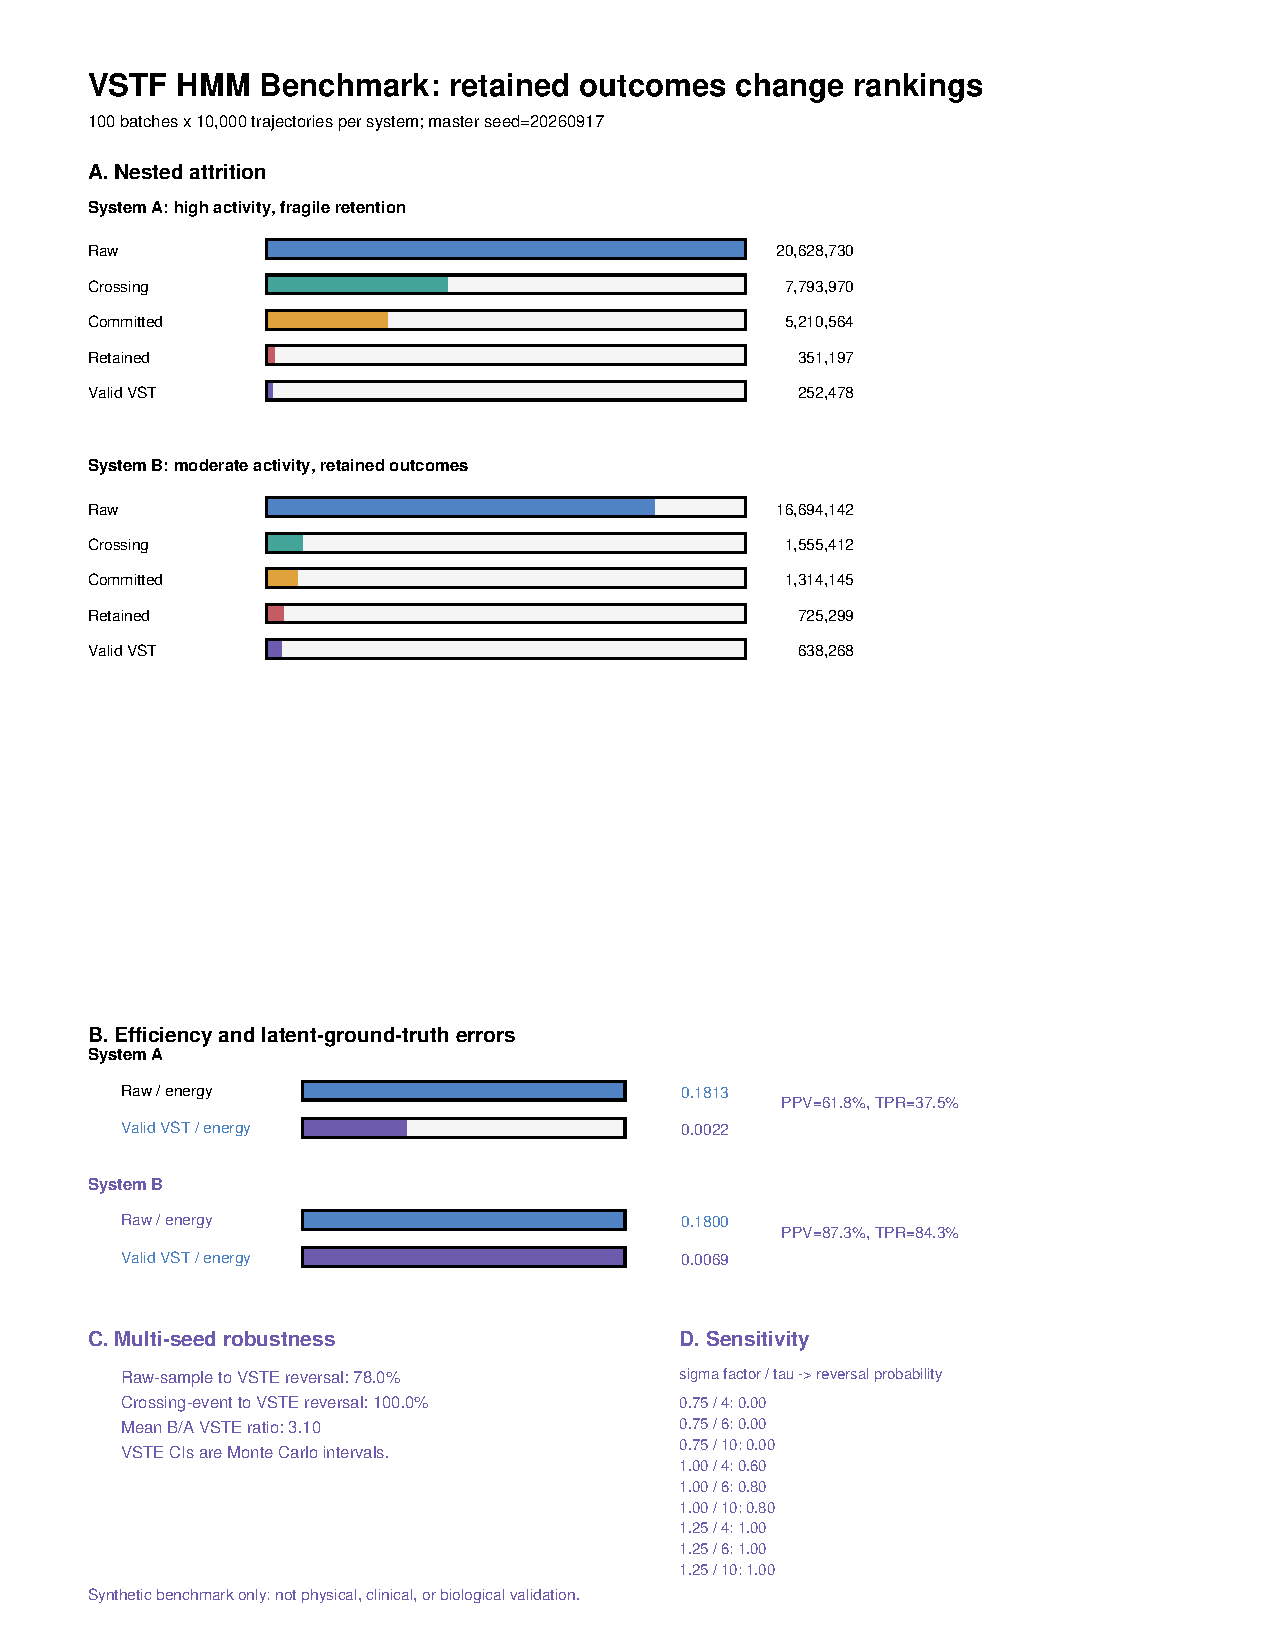
\includegraphics[width=0.96\linewidth]{vstf_hmm_benchmark.pdf}
\caption{Hidden-Markov benchmark showing nested attrition from raw activity to valid VST events. System A produces more raw activity per supplied energy, but most committed events fail validation or retention. System B produces fewer raw events but substantially higher valid VST yield per supplied energy.}
\end{figure}

\begin{table}[h]
\centering
\caption{Summary of the 10,000-trajectory HMM benchmark.}
\begin{tabular}{lrr}
\toprule
Quantity & System A & System B \\
\midrule
Raw activity & 205,878 & 167,112 \\
Crossing events & 78,013 & 15,477 \\
Committed events & 52,170 & 13,099 \\
Retained events & 3,467 & 7,257 \\
Valid VST events & 2,491 & 6,433 \\
False successes & 46,152 & 5,385 \\
Pending/right-censored events & 3,527 & 1,281 \\
Full-boundary energy & 1,137,683 & 927,206 \\
Raw activity per energy & 0.18096 & 0.18023 \\
Valid VST per energy & 0.00219 & 0.00694 \\
Retention yield & 0.066 & 0.554 \\
False-success fraction & 0.885 & 0.411 \\
\bottomrule
\end{tabular}
\end{table}

The raw-activity ranking and VSTF ranking disagree. System A is slightly higher on raw activity per supplied energy, while System B is more than three times higher on valid VST per supplied energy. This is precisely the incremental claim VSTF must earn: the acceptance layer can remove false successes and reverse or materially alter rankings that would be drawn from raw activity, crossings, or committed first-passage events alone.

\section{Reproducibility Materials}

The synthetic benchmark is intended to be fully reproducible. The required companion files are:
\begin{itemize}
  \item \href{https://github.com/MartinPetrasek123/R_Universe_Evidence_Audited/blob/main/vstf/vstf_hmm_benchmark.py}{\texttt{vstf\_hmm\_benchmark.py}}: deterministic simulation script with fixed seed, model parameters, event filters, and figure generation.
  \item \href{https://github.com/MartinPetrasek123/R_Universe_Evidence_Audited/blob/main/vstf/vstf_hmm_benchmark_summary.csv}{\texttt{vstf\_hmm\_benchmark\_summary.csv}}: aggregate benchmark output used in Table 3.
  \item \href{https://github.com/MartinPetrasek123/R_Universe_Evidence_Audited/blob/main/vstf/vstf_hmm_benchmark.pdf}{\texttt{vstf\_hmm\_benchmark.pdf}}: generated benchmark figure used in Figure 1.
\end{itemize}
When the manuscript is hosted in a public repository, these links should resolve to the repository copies of the files. The benchmark does not require domain data and is not evidence for a biological or clinical claim; it is a reproducible methodological demonstration that the VSTF acceptance layer can alter ranking and false-success interpretation.

\section{Operational Workflow}

A VSTF study should be executable as the following locked workflow.

\begin{enumerate}
  \item \textbf{Define the scientific claim.} State whether the claim concerns event detection, retained outcome, cost-normalized efficiency, clinical prediction, intervention response, or causal treatment benefit.
  \item \textbf{Declare the state representation.} Specify $X_t$, measured data $Y_t$, preprocessing, feature construction, and the observation model or measurement-error approximation.
  \item \textbf{Freeze state regions.} Define $C_i$ and $C_j$ using prior knowledge or a training/reference cohort. Lock them before confirmatory testing.
  \item \textbf{Freeze event segmentation.} Specify departure, commitment, dwell, exit, return, hysteresis, refractory time, and double-counting rules.
  \item \textbf{Freeze validity predicates.} Declare localization, distinguishability, persistence or resilience, and $V_{\mathrm{dom}}$ thresholds.
  \item \textbf{Declare boundary and denominator.} Define $\mathcal{B}$ and decide which costs, attempts, readouts, rejected events, and stabilization periods are included.
  \item \textbf{Run baseline models.} Compare against raw activity, raw crossings, first-passage counts, TPT/Markov-state rates, ordinary yield, or standard prediction models.
  \item \textbf{Estimate VST observables.} Report hard counts, probabilistic counts, finite-window rates, cost-normalized yields, uncertainty, and threshold sensitivity.
  \item \textbf{Assign claim level.} Label the result as proxy, task-level, or fully measured VST. Do not claim causal benefit unless a causal design supports it.
  \item \textbf{Release reproducibility materials.} Provide code, thresholds, state-region definitions, event lists, rejected-event counts, and denominator ledgers.
\end{enumerate}

\section{Three Levels of Evidence}

VSTF requires separation of evidence levels.

\begin{table}[h]
\centering
\caption{Evidence levels for valid transition claims.}
\begin{tabular}{p{0.22\linewidth}p{0.34\linewidth}p{0.34\linewidth}}
\toprule
Level & What is measured & What cannot be claimed \\
\midrule
Proxy VST & Public or incomplete data satisfy an approximate event rule. & Full physical or causal validation. \\
Task-level VST & A benchmark or protocol defines completed outcomes and energy per task. & Microscopic entropy production or retention unless measured. \\
State-valid VST & Localization, distinguishability, event-level retention or declared resilience, and admissible domain validity are measured under a locked protocol. & Energy-normalized efficiency or cross-system cost comparison without complete denominator accounting. \\
Cost-accounted VST & State-valid VST plus complete window-level denominator accounting $Q_{\mathcal{B}}^{\mathrm{acct}}[a,b]=1$. & Causal treatment benefit or generalization beyond the tested boundary without separate validation. \\
\bottomrule
\end{tabular}
\end{table}

\section{Domain Instantiations}

\subsection{Computational Hardware}

For VLSI, edge-AI, stochastic devices, memory cells, or quantum readout systems, define state regions as accepted output classes, memory states, pointer states, or retained device states.

An event is valid only if:
\begin{enumerate}
  \item the output is localized in a declared class,
  \item distinguishability exceeds the readout threshold,
  \item retention persists over $\tau_\ast$,
  \item rejected attempts remain in the energy denominator,
  \item quality or correctness predicates are passed.
\end{enumerate}

At this layer, VSTF recovers the logic of the Valid Irreversible Resolution Rate:
\[
  \VIRR = \frac{R_{\mathrm{valid}}}{P}.
\]
The contribution is not arithmetic novelty when public benchmarks already report energy per task or full-system power \cite{mlperf}. The contribution is the explicit event boundary, the accepted-outcome denominator, and the refusal to count raw activity as an accepted retained outcome.

\noindent\textbf{Minimum confirmatory hardware protocol.}
\begin{enumerate}
  \item Freeze task definition, input distribution, correctness criterion, retention window, and readout method.
  \item Count all candidate attempts, not only successful outputs.
  \item Measure full-system energy at the declared boundary, including host, memory, conversion, calibration, readout, and failed attempts when inside $\mathcal{B}$.
  \item Report raw operations per watt, accepted outputs per watt, retained accepted outputs per watt, and error burden.
  \item Test whether VSTF changes ranking against a standard benchmark denominator.
\end{enumerate}

The hardware claim is falsified if accepted-output yield is not materially different from ordinary benchmark yield after full-boundary accounting, or if failures are already fully captured by the benchmark's native validity rules.

\subsection{Physiological Stability}

Two distinct ICU uses must not be conflated. In a \emph{patient-state VST}, $X_t$ is the latent physiological state of the patient and the prediction model estimates a patient transition. In a \emph{decision-state VST}, $X_t$ is the state of an alarm, triage, or clinical decision system. Both are legitimate, but a manuscript must declare which ontology is being evaluated.

In intensive-care time series, let
\[
  x(t)=[\mathrm{HR},\mathrm{MAP},\mathrm{RR},\mathrm{SpO}_2,\mathrm{Temp},\ldots]
\]
and define dynamic components:
\[
  P(t) = \mathrm{perturbation\ intensity},\quad
  A(t) = \mathrm{autocorrelation\ persistence},
\]
\[
  R(t) = \mathrm{relaxation\ proxy},\quad
  D_C(t)=\mathrm{coupling\ change}.
\]

For patient-state use, the physiological stability framework becomes a VSTF problem only when an elevated dynamic state is linked to a valid patient-level transition under locked rules:
\[
  \mathrm{dynamic\ change} \longrightarrow \mathrm{validated\ patient\ transition}.
\]
For decision-state use, the VST event is the accepted alarm or decision transition, not the patient's biological transition itself. Until patient-level calibration, raw-vital baselines, alarm burden, decision curves, and external validation are completed, PSI-like outputs should be treated as component-level instability features rather than clinical VST events. A minimal clinical validation panel should include calibration-in-the-large, calibration slope or curve, discrimination, Brier score, net benefit, alarm burden, and an explicit baseline such as NEWS2 or a raw-vital model \cite{news2,trwscore,physionet,harutyunyan2019}. Reporting should follow current prediction-model standards, including TRIPOD, TRIPOD+AI, PROBAST+AI, and REMARK where applicable \cite{remark,tripod,collins2024tripodai,moons2025probastai}.

\noindent\textbf{Minimum confirmatory ICU protocol.}
\begin{enumerate}
  \item Freeze the clinical endpoint, prediction horizon, exclusion rules, preprocessing, and alarm threshold.
  \item Split development, calibration, and external validation cohorts by hospital, unit, or time period where possible.
  \item Compare against NEWS2, raw vital signs, and a standard time-series baseline.
  \item Report calibration, discrimination, Brier score, net benefit, alarm burden, false alarms per patient-day, and missed-event rate.
  \item Treat a PSI-like signal as a VST event only when it changes externally validated patient-level prediction or decision utility.
\end{enumerate}

The clinical VST claim is falsified if dynamic coupling features do not improve externally validated prediction or utility beyond simpler baselines.

\subsection{Pathological Tumor-State Reset}

For tumor systems, where wound-repair analogies and modern hallmarks motivate state-based descriptions of malignancy \cite{dvorak1986,hanahan2011}, define a module vector
\[
  x(t)=
  [S_{\mathrm{ECM}},S_{\mathrm{hypoxia}},S_{\mathrm{proteostasis}},S_{\mathrm{alarm}},
  C_{\mathrm{junction}},C_{\mathrm{polarity}},C_{\mathrm{circadian}},C_{\mathrm{mitochondrial}},\ldots].
\]

Here \OSD{} is used only as a declared multivariate organism-stability-disruption score derived from pre-specified molecular modules. It is not assumed to be a universal cancer mechanism. A safer biological term is \emph{pathological tumor-state} unless a wound-repair signature is explicitly part of the module definition.

Let $x_{\mathrm{path}}$ be the baseline pathological tumor-state vector and $x_{\mathrm{ref}}$ a frozen low-\OSD{} or normal-like reference. Define
\[
  D_{\mathrm{path}}(t)=
  (x(t)-\mu_{\mathrm{path}})^\top\Sigma^{-1}(x(t)-\mu_{\mathrm{path}}),
  \qquad
  D_{\mathrm{ref}}(t)=
  (x(t)-\mu_{\mathrm{ref}})^\top\Sigma^{-1}(x(t)-\mu_{\mathrm{ref}}),
\]
\[
  Y(t)=D_{\mathrm{path}}(t)-D_{\mathrm{ref}}(t).
\]
Here $\mu_{\mathrm{path}}$, $\mu_{\mathrm{ref}}$, feature scaling, module definitions, and covariance estimate $\Sigma$ must be frozen from an independent training/reference cohort before confirmatory testing. If the number of features is not small relative to the training cohort, $\Sigma^{-1}$ must be estimated with a pre-specified shrinkage, diagonal, low-rank, or regularized covariance protocol.

A reset transition is valid only if the post-rechallenge state remains displaced away from $x_{\mathrm{path}}$ and toward $x_{\mathrm{ref}}$ after withdrawal:
\[
  \Delta_{\mathrm{path}}
  =
  D_{\mathrm{path}}(T4)-D_{\mathrm{path}}(T0)
  \geq \eta_{\mathrm{path}},
  \qquad
  \Delta_{\mathrm{ref}}
  =
  D_{\mathrm{ref}}(T0)-D_{\mathrm{ref}}(T4)
  \geq \eta_{\mathrm{ref}},
\]
with viability, target engagement, clone-selection controls, and locked module definitions. The scalar contrast $Y(t)=D_{\mathrm{path}}(t)-D_{\mathrm{ref}}(t)$ may be reported as a secondary summary, but it is not sufficient by itself because it can improve through movement in only one direction.

Acute cytotoxicity is not a valid reset by itself. The primary confirmatory analysis should estimate a treatment-by-time effect with biological-replicate or clone-level random effects, rather than relying only on the sign of a single post-treatment difference. This is consistent with modern work on therapy-induced cancer-cell state transitions and persister lineages \cite{oren2021}.

\noindent\textbf{Minimum confirmatory cancer protocol.}
\begin{enumerate}
  \item Freeze module definitions, normalization, reference cohorts, covariance/shrinkage method, and reset threshold before testing.
  \item Include vehicle, cytotoxic-positive, pathway-specific, withdrawal, and rechallenge conditions.
  \item Distinguish cell killing from surviving-cell state reset by measuring viable surviving populations.
  \item Control for clone selection, lineage effects, batch effects, and proliferation-rate artifacts.
  \item Use a longitudinal model with treatment, time, treatment-by-time interaction, and replicate or clone effects.
\end{enumerate}

The reset claim is falsified if the apparent improvement disappears after withdrawal, rechallenge, viable-survivor analysis, or clone-selection control.

\subsection{Neurorehabilitation}

Let
\[
  x(t)=[U(t),E(t),M(t),Y(t),S_f(t),A_u(t),B_p(t)]
\]
represent voluntary intent, stimulation, EMG, movement, sensory feedback, autonomic state, and pain/spasticity/fatigue.

A motor event is provisionally valid only if movement depends on intent under stimulation:
\[
  \Pr(Y=1\mid U=1,E=1)>\Pr(Y=1\mid U=0,E=1),
\]
or more strongly,
\[
  I(U;Y\mid E,P_{\mathrm{body}},T_{\mathrm{session}})>0.
\]
These inequalities establish conditional dependence, not by themselves causal voluntary control. A confirmatory design should use randomized cue epochs, sham or no-intent epochs, artifact masking, pre-specified lag windows, and clustered inference by participant and session. A compact model is
\[
  \mathrm{logit}\,\Pr(Y=1)
  =
  \beta_0+\beta_U U+\beta_E E+\beta_{UE}(U\times E)+\beta_Z Z,
\]
where $Z$ contains posture, cue timing, prior stimulation, fatigue, and artifact controls.
The intent variable $U$ must be measured independently of the movement outcome used to define $Y$; otherwise intent-outcome coupling can become circular. A minimum clinically meaningful effect-size margin for $\beta_{UE}$ or the corresponding risk difference should be specified before testing.

Retention requires:
\[
  \Pr(Y=1\mid U=1,E=0,\mathrm{post})
  >
  \Pr(Y=1\mid U=1,E=0,\mathrm{baseline}).
\]

Thus a stimulation-evoked contraction is not a valid functional transition unless it is localized, distinguishable from artifact or reflex, stable or retained over an operational window, and coupled to voluntary intent. Off-stimulation post-training performance should be reported as a separate retention endpoint. Human spinal-cord stimulation studies and work on metastable neural dynamics provide useful precedents because they explicitly separate stimulation-supported movement, voluntary control, proprioceptive constraints, retained post-training function, and circuit-state dynamics \cite{brinkman2022,wagner2018,formento2018}.

\noindent\textbf{Minimum confirmatory neurorehabilitation protocol.}
\begin{enumerate}
  \item Randomize cue, intent, sham, stimulation, and no-intent epochs where ethically and practically possible.
  \item Measure voluntary intent independently of the movement endpoint and predefine a minimum effect-size margin.
  \item Predefine lag windows between intent, stimulation, EMG, and movement.
  \item Mask or model stimulation artifacts, reflex responses, posture, fatigue, pain, spasticity, and session effects.
  \item Report stimulation-on performance separately from stimulation-off post-training retention.
  \item Use participant- and session-clustered inference rather than treating repeated movement attempts as independent.
\end{enumerate}

The voluntary-control claim is falsified if movement is equally explained by stimulation timing, artifact, posture, reflex, or cue structure without independent contribution from voluntary intent.

\section{General Falsification Criteria}

\begin{criterion}[Baseline sufficiency]
If a simpler baseline model explains the outcome with equal or better performance under the same validation procedure, the VST-specific claim is not supported.
\end{criterion}

\begin{criterion}[Antecedent sufficiency]
If a standard TPT, first-passage, Markov-state, reliability-yield, or clinical-validation model captures the claimed result without the VSTF acceptance layer changing inference, ranking, or decision utility, then the incremental VSTF claim is not supported.
\end{criterion}

\begin{criterion}[Event-rule failure]
If localization, distinguishability, persistence or resilience, accounting quality, or the domain predicate cannot be measured or fails under a locked protocol, only a proxy claim is allowed.
\end{criterion}

\begin{criterion}[Post-hoc threshold failure]
If the operating threshold is selected after outcome inspection and not revalidated prospectively, the result is exploratory.
\end{criterion}

\begin{criterion}[No-retention failure]
If the state moves during perturbation but returns to the original basin after withdrawal or rechallenge, the event is activity or response, not a valid stabilized transition.
\end{criterion}

\begin{criterion}[Boundary failure]
If major energy, dose, rejected attempts, readout, or stabilization costs are excluded from the declared denominator, energy-normalized claims are invalid for cross-system comparison.
\end{criterion}

\begin{criterion}[Accounting-validity separation]
If a candidate event passes localization, distinguishability, persistence, and domain validity but lacks a complete cost ledger, it may be reported as a state-valid event but cannot support \VSTE{}, cost-yield, or cross-system efficiency claims.
\end{criterion}

\section{Reporting Standard}

Every VSTF study should report:

\begin{enumerate}
  \item state variables and preprocessing rules,
  \item operational state regions $C_i$,
  \item whether $C_i$ were fixed a priori or estimated from a training/reference cohort,
  \item observation model $P_M(Y\mid X)$ or a justified measurement-error approximation,
  \item candidate-event segmentation: origin, departure, commitment, end, hysteresis, refractory interval, and double-counting rule,
  \item event index timestamp and right-censoring rule for finite windows,
  \item measurement map and distinguishability threshold or error criterion,
  \item latent process model $(p_0,K_\theta,P_M)$ or calibrated classifier-localization procedure,
  \item persistence window $\tau_\ast$ and first-exit or return-time rule,
  \item domain validity predicate,
  \item admissibility justification for $V_{\mathrm{dom}}$,
  \item event-granularity comparability or sensitivity analysis,
  \item system boundary and energy or perturbation ledger,
  \item accounting-quality flag $Q^{\mathrm{acct}}$,
  \item window-level denominator-completeness flag $Q_{\mathcal{B}}^{\mathrm{acct}}[a,b]$,
  \item accepted and rejected candidate counts,
  \item baseline models and negative controls,
  \item uncertainty analysis and dependence corrections,
  \item sensitivity to $\epsilon$, $\alpha$, $\delta$, $\tau_\ast$, segmentation, and domain thresholds,
  \item exact code or command-level reproducibility path,
  \item explicit claim level: proxy, task-level, state-valid, or cost-accounted VST.
\end{enumerate}

\section{Preregisterable Hypotheses}

\begin{hypothesis}[Ranking reversal under full cost boundaries]
In a benchmark population of systems with matched raw activity efficiency, the ranking induced by $\widehat{\VSTE}$ will differ from the ranking induced by raw activity per watt after rejected attempts, retention failures, readout, and stabilization overhead are included.

\noindent\textbf{Primary statistic.} For $m$ systems, define the fraction of discordant pairs
\[
  D=
  \frac{
  \sum_{i<j}
  \1\{\mathrm{sgn}(R_i-R_j)\neq \mathrm{sgn}(V_i-V_j)\}
  }{\binom{m}{2}},
\]
where $R_i$ is raw activity efficiency and $V_i$ is $\widehat{\VSTE}$ for system $i$. Ties must be handled by a locked rule.

\noindent\textbf{Null hypothesis.} $H_0:D\leq D_{\min}$, where $D_{\min}$ is the minimum scientifically relevant discordant-pair fraction.

\noindent\textbf{Falsification rule.} If $D$ does not exceed $D_{\min}$ with pre-specified uncertainty control, or if discordant ranking changes are not reproducible in an external benchmark set, the VSTF ranking-reversal claim is not supported for that domain.
\end{hypothesis}

\begin{hypothesis}[Coupling over amplitude]
In complex biological time series, models containing pre-specified coupling-change variables will improve externally validated prediction of fully measured VST events over amplitude-only models.

\noindent\textbf{Primary endpoint.} The primary endpoint should be declared in advance, for example $\Delta$Brier score for probabilistic prediction or $\Delta$net benefit over a pre-specified decision-threshold range for clinical decision support. Calibration, discrimination, and alarm burden should be secondary endpoints unless declared primary.

\noindent\textbf{Null hypothesis.} Coupling variables do not improve the pre-specified primary endpoint beyond an amplitude-only baseline in external validation.

\noindent\textbf{Falsification rule.} If improvement is absent after external validation, uncertainty estimation, and multiplicity control for secondary endpoints, the coupling claim is rejected for that setting.
\end{hypothesis}

\begin{hypothesis}[Retention attrition after acute response]
In perturbation experiments, acute response does not imply durable reset. Among acute candidate responses, define
\[
  p_{\mathrm{ret}}=\Pr(\mathrm{retained\ reset}\mid \mathrm{acute\ response}).
\]

\noindent\textbf{Null hypothesis.} $H_0:p_{\mathrm{ret}}\geq 1-\rho_\ast$, where $\rho_\ast$ is a pre-specified maximum acceptable attrition margin. Alternatively, compare two protocols by testing $p_{\mathrm{ret}}^{(A)}=p_{\mathrm{ret}}^{(B)}$.

\noindent\textbf{Falsification rule.} If acute responses are retained after withdrawal and rechallenge with attrition below the pre-specified margin, or if no protocol-level difference in $p_{\mathrm{ret}}$ is observed where predicted, the VSTF reset-vs-response claim is unsupported for that protocol.
\end{hypothesis}

\begin{conjecture}[Decision-loop bottleneck]
In computational architectures dominated by measurement, branching, synchronization, readout, or feedback, reducing pre-specified decision-loop closures may improve accepted outcome yield more than increasing raw internal activity at fixed decision overhead. Let
\[
  C_{\mathrm{loop}}
\]
denote a locked count of branch, readout, synchronization, or feedback closures for a declared workload. This conjecture becomes a preregisterable hypothesis only when an intervention changes $C_{\mathrm{loop}}$ while holding architecture, memory traffic, throughput target, and error tolerance sufficiently fixed.

\noindent\textbf{Null hypothesis for a future test.} Accepted outcome yield is explained fully by raw internal activity, throughput, error rate, memory traffic, and full-system energy, with no additional contribution from $C_{\mathrm{loop}}$.

\noindent\textbf{Falsification rule.} If decision-loop reductions do not improve $\widehat{\VSTE}$ after controlling for throughput, error rate, memory traffic, and full-system power, the bottleneck claim is not supported.
\end{conjecture}

\section{Limitations}

\begin{limitation}[Coarse-graining dependence]
VST observables depend on the chosen state partition. This is not a defect if the partition is declared, justified, and stress-tested. It is a defect if partitions are tuned after outcome inspection.
\end{limitation}

\begin{limitation}[Domain specificity]
The validity predicate is domain-specific. A universal mathematical skeleton does not imply a universal biological or physical mechanism.
\end{limitation}

\begin{limitation}[No automatic causality]
Retrospective association between a score and an endpoint does not establish that the score causes, controls, or can prevent the transition.
\end{limitation}

\begin{limitation}[No scalar absolutism]
The framework does not require a single universal scalar. In many domains, the correct output is a tuple: rate, energy-normalized yield, retention, false-event burden, and component attribution.
\end{limitation}

\section{Ethical Scope of Future Validation}

This manuscript is a theoretical and methodological synthesis and uses no new human or animal data. Therefore, institutional review-board or animal-care approval is not required for the manuscript itself.

Future ICU, oncology, neurorehabilitation, or animal-tumor validation studies would require their own ethical review. Human studies should specify informed consent or waiver, privacy protection for identifiable data, adverse-event monitoring, and fairness analysis when prediction models may affect clinical decisions. Animal studies should follow ARRIVE 2.0 reporting principles and justify sample size, randomization, blinding, exclusions, and humane endpoints \cite{arrive2020}. In all clinical applications, measurement validity, predictive validity, clinical utility, and causal treatment benefit must be reported as separate claims.

\section{Claim Audit and Reviewer-Safe Interpretation}

The framework is easiest to overstate in four places. The following interpretations are therefore part of the formal manuscript rather than informal caveats.

\subsection{Novelty Claim}

VSTF does not claim to discover transition paths, state basins, event rates, or first-exit processes. Its novelty is the cross-domain acceptance grammar that determines when a dynamically detected event becomes a countable outcome under locked validity and cost rules. If a domain already has an equivalent acceptance grammar, VSTF should be described as a translation or unification, not as a new mechanism.

\subsection{Thermodynamic Claim}

VSTF does not assign a universal Landauer cost to every biological, clinical, or computational event. Landauer-type bounds apply only to logically irreversible information operations under the relevant assumptions. For other systems, energy, entropy, dose, or risk burden are denominators for accountable comparison, not universal physical lower bounds.

Thermodynamic work/free-energy relations are treated as conditional physical specializations. The general VSTF metric is an engineering or methodological ratio of accepted retained outcomes to a declared denominator. It remains meaningful even when no microscopic thermodynamic lower bound is asserted.

\subsection{Clinical Claim}

VSTF does not allow a dynamic instability score to be called a clinical event. A clinical VST requires external validation, calibration, utility assessment, and comparison with simpler baselines. Measurement validity, prediction validity, decision utility, and treatment benefit are distinct layers.

\subsection{Biological Mechanism Claim}

VSTF does not assert that cancer reset, physiological stabilization, and motor recovery share one biological mechanism. It asserts only that all three can be evaluated using the same event-level grammar: state localization, distinguishability, retention, domain validity, and accountable denominator. Terms such as repair-like state, tumor-state reset, or organism-stability disruption must be operationally defined in each biological study.

\subsection{What Would Make VSTF Scientifically Unnecessary}

VSTF would add little if, across representative domains, accepted-transition counts never differ from raw activity, first-passage counts, standard yield metrics, or ordinary validated prediction models. The framework earns its place only when the acceptance layer changes ranking, interpretation, rejection of false successes, or protocol design.

\section{Discussion}

The central move of VSTF is simple: change the counted object. Many existing frameworks ask how much energy is used, how much entropy is produced, how much information is transmitted, how much activity occurs, or how large a score becomes. VSTF asks whether the system produced a valid stabilized transition.

This reframing is valuable because it separates activity from outcome. A dissipative process may produce no accepted transition. A high-throughput device may fail retention. A tumor perturbation may kill cells without resetting surviving state dynamics. A neuromodulation protocol may evoke movement without voluntary control. A physiological score may detect weak instability without clinical utility.

The framework is strongest where the four state-validity predicates and the accounting-quality flag can all be measured under a locked protocol. It is weakest when only proxy features exist. The intended use is therefore not rhetorical unification but disciplined experimental design.

\section{Conclusion}

The Valid State Transition Framework formalizes a cross-domain measurement principle: count stabilized, distinguishable, valid transitions rather than raw activity. The framework is compatible with thermodynamics, stochastic trajectories, critical-transition theory, clinical model validation, and systems biology, but it does not replace them. Its contribution is operational and falsifiable.

The practical question becomes:
\[
  \text{How many valid stabilized state transitions does the system produce per unit cost?}
\]

This question can be applied to hardware, physiological monitoring, cancer-state reset experiments, neurorehabilitation, and other systems where transient activity and durable outcome are easily confused. The framework should advance only where locked protocols, baseline comparisons, negative controls, and reproducible ledgers show that it adds information beyond simpler explanations.

\section*{Declarations}

\textbf{Funding.} No external funding is declared in this draft.

\textbf{Competing interests.} The author declares no competing interests.

\textbf{Data and code availability.} This manuscript is a theoretical and methodological synthesis with a synthetic HMM demonstration. The simulation script, summary table, and figure are provided as \texttt{vstf\_hmm\_benchmark.py}, \texttt{vstf\_hmm\_benchmark\_summary.csv}, and \texttt{vstf\_hmm\_benchmark.pdf}. Domain-specific empirical claims require separate reproducibility packages, locked datasets, code, and analysis logs.

\textbf{Author contribution.} M. Petrasek conceived the framework, integrated prior theoretical and applied components, and wrote the manuscript.

\begin{thebibliography}{99}

\bibitem{landauer1961}
R. Landauer.
Irreversibility and heat generation in the computing process.
\emph{IBM Journal of Research and Development}, 5(3):183--191, 1961.

\bibitem{bennett2003}
C. H. Bennett.
Notes on Landauer's principle, reversible computation, and Maxwell's demon.
\emph{Studies in History and Philosophy of Modern Physics}, 34(3):501--510, 2003.

\bibitem{berut2012}
A. Berut, A. Arakelyan, A. Petrosyan, S. Ciliberto, R. Dillenschneider, and E. Lutz.
Experimental verification of Landauer's principle linking information and thermodynamics.
\emph{Nature}, 483:187--189, 2012.

\bibitem{seifert2005}
U. Seifert.
Entropy production along a stochastic trajectory and an integral fluctuation theorem.
\emph{Physical Review Letters}, 95:040602, 2005.

\bibitem{seifert2012}
U. Seifert.
Stochastic thermodynamics, fluctuation theorems and molecular machines.
\emph{Reports on Progress in Physics}, 75:126001, 2012.

\bibitem{barato2015}
A. C. Barato and U. Seifert.
Thermodynamic uncertainty relation for biomolecular processes.
\emph{Physical Review Letters}, 114:158101, 2015.

\bibitem{jarzynski1997}
C. Jarzynski.
Nonequilibrium equality for free energy differences.
\emph{Physical Review Letters}, 78(14):2690--2693, 1997.

\bibitem{sagawa2010}
T. Sagawa and M. Ueda.
Generalized Jarzynski equality under nonequilibrium feedback control.
\emph{Physical Review Letters}, 104:090602, 2010.

\bibitem{kramers1940}
H. A. Kramers.
Brownian motion in a field of force and the diffusion model of chemical reactions.
\emph{Physica}, 7(4):284--304, 1940.

\bibitem{e2006}
W. E and E. Vanden-Eijnden.
Towards a theory of transition paths.
\emph{Journal of Statistical Physics}, 123:503--523, 2006.

\bibitem{metzner2009}
P. Metzner, C. Schutte, and E. Vanden-Eijnden.
Transition path theory for Markov jump processes.
\emph{Multiscale Modeling \& Simulation}, 7(3):1192--1219, 2009.

\bibitem{scheffer2009}
M. Scheffer, J. Bascompte, W. A. Brock, V. Brovkin, S. R. Carpenter, V. Dakos, H. Held,
E. H. van Nes, M. Rietkerk, and G. Sugihara.
Early-warning signals for critical transitions.
\emph{Nature}, 461:53--59, 2009.

\bibitem{scheffer2018}
M. Scheffer, J. E. Bolhuis, D. Borsboom, T. G. Buchman, S. M. W. Gijzel, D. Goulson,
J. E. Kammenga, B. Kemp, I. A. van de Leemput, S. Levin, C. M. Martin, R. J. F. Melis,
E. H. van Nes, L. M. Romero, and M. G. M. Olde Rikkert.
Quantifying resilience of humans and other animals.
\emph{Proceedings of the National Academy of Sciences}, 115(47):11883--11890, 2018.

\bibitem{dvorak1986}
H. F. Dvorak.
Tumors: wounds that do not heal. Similarities between tumor stroma generation and wound healing.
\emph{New England Journal of Medicine}, 315(26):1650--1659, 1986.

\bibitem{hanahan2011}
D. Hanahan and R. A. Weinberg.
Hallmarks of cancer: the next generation.
\emph{Cell}, 144(5):646--674, 2011.

\bibitem{oren2021}
Y. Oren, M. Tsabar, M. S. Cuoco, L. Amir-Zilberstein, H. F. Cabanos, J.-C. Hutter,
B. Hu, and colleagues.
Cycling cancer persister cells arise from lineages with distinct programs.
\emph{Nature}, 596:576--582, 2021.

\bibitem{brinkman2022}
B. A. W. Brinkman, H. Yan, A. Maffei, I. M. Park, A. Fontanini, J. Wang, and G. La Camera.
Metastable dynamics of neural circuits and networks.
\emph{Applied Physics Reviews}, 9(1):011313, 2022.

\bibitem{wagner2018}
F. B. Wagner, J.-B. Mignardot, C. G. Le Goff-Mignardot, R. Demesmaeker, S. Komi,
and colleagues.
Targeted neurotechnology restores walking in humans with spinal cord injury.
\emph{Nature}, 563:65--71, 2018.

\bibitem{formento2018}
E. Formento, K. Minassian, F. B. Wagner, J.-B. Mignardot, C. G. Le Goff-Mignardot,
A. Rowald, and colleagues.
Electrical spinal cord stimulation must preserve proprioception to enable locomotion in humans with spinal cord injury.
\emph{Nature Neuroscience}, 21:1728--1741, 2018.

\bibitem{sturmberg2014}
J. P. Sturmberg, C. M. Martin, and D. A. Katerndahl.
Systems and complexity thinking in the general practice literature: an integrative, historical narrative review.
\emph{Annals of Family Medicine}, 12(1):66--74, 2014.

\bibitem{news2}
Royal College of Physicians.
\emph{National Early Warning Score (NEWS) 2: Standardising the assessment of acute-illness severity in the NHS}.
Updated report, 2017.

\bibitem{trwscore}
T. Desautels, J. Calvert, J. Hoffman, M. Jay, Y. Kerem, L. Shieh, D. Shimabukuro, U. Chettipally, M. D. Feldman, C. Barton, D. J. Wales, and R. Das.
Prediction of sepsis in the intensive care unit with minimal electronic health record data: a machine learning approach.
\emph{JMIR Medical Informatics}, 4(3):e28, 2016.

\bibitem{physionet}
A. L. Goldberger, L. A. N. Amaral, L. Glass, J. M. Hausdorff, P. C. Ivanov, R. G. Mark,
J. E. Mietus, G. B. Moody, C.-K. Peng, and H. E. Stanley.
PhysioBank, PhysioToolkit, and PhysioNet: components of a new research resource for complex physiologic signals.
\emph{Circulation}, 101(23):e215--e220, 2000.

\bibitem{harutyunyan2019}
H. Harutyunyan, H. Khachatrian, D. C. Kale, G. Ver Steeg, and A. Galstyan.
Multitask learning and benchmarking with clinical time series data.
\emph{Scientific Data}, 6:96, 2019.

\bibitem{mlperf}
V. J. Reddi et al.
MLPerf Inference Benchmark.
In \emph{Proceedings of the ACM/IEEE International Symposium on Computer Architecture}, pages 446--459, 2020.

\bibitem{phillips2014}
S. D. Phillips and M. Krystek.
Assessment of conformity, decision rules and risk analysis.
\emph{Technisches Messen}, 81(5):227--234, 2014.

\bibitem{jcgm106}
Joint Committee for Guides in Metrology.
\emph{JCGM 106:2012: Evaluation of measurement data -- The role of measurement uncertainty in conformity assessment}.
JCGM, 2012.

\bibitem{remark}
L. M. McShane, D. G. Altman, W. Sauerbrei, S. E. Taube, M. Gion, and G. M. Clark.
Reporting recommendations for tumor marker prognostic studies.
\emph{Journal of Clinical Oncology}, 23(36):9067--9072, 2005.

\bibitem{tripod}
G. S. Collins, J. B. Reitsma, D. G. Altman, and K. G. M. Moons.
Transparent reporting of a multivariable prediction model for individual prognosis or diagnosis (TRIPOD).
\emph{Annals of Internal Medicine}, 162(1):55--63, 2015.

\bibitem{collins2024tripodai}
G. S. Collins, K. G. M. Moons, P. Dhiman, R. D. Riley, A. L. Beam, B. Van Calster,
M. Ghassemi, X. Liu, J. B. Reitsma, M. van Smeden, and colleagues.
TRIPOD+AI statement: updated guidance for reporting clinical prediction models that use regression or machine learning methods.
\emph{BMJ}, 385:e078378, 2024.

\bibitem{moons2025probastai}
K. G. M. Moons, J. A. A. Damen, T. Kaul, L. Hooft, C. Andaur Navarro, P. Dhiman,
and colleagues.
PROBAST+AI: an updated quality, risk of bias, and applicability assessment tool for prediction models using regression or artificial intelligence methods.
\emph{BMJ}, 388:e082505, 2025.

\bibitem{arrive2020}
N. Percie du Sert, V. Hurst, A. Ahluwalia, S. Alam, M. T. Avey, M. Baker,
W. J. Browne, and colleagues.
The ARRIVE guidelines 2.0: updated guidelines for reporting animal research.
\emph{PLOS Biology}, 18(7):e3000410, 2020.

\end{thebibliography}

\end{document}
